%% For Page Style :
\pagestyle{fancy}
\fancyhf{}
\fancyhead[LE]{\thepage}
\fancyhead[RO]{\thepage}
\fancyhead[RE]{\nouppercase{\textbf{\leftmark}}}
\fancyhead[LO]{\textbf{Tutorial BlankOnDev version 0.1005}}
\setlength{\parindent}{1cm}
\setlength{\parskip}{0.25cm}
%\fontsize{\normalsize}{baselineskip}

%% Format Chapter
\definecolor{RoyalRed}{RGB}{157,16, 45}
\chapterfont{\fontfamily{bch}\fontseries{b}\selectfont}

\titleformat{\chapter}[display]
{\normalfont\bfseries\filcenter}
{\LARGE}
{1ex}
{\titlerule[2pt]
	\textbf{{\LARGE \thechapter} \hspace{1mm}\textbf{{\LARGE |}}}
	\hspace{1mm}%
	\LARGE}
[\vspace{1ex}%
{\titlerule[2pt]}]
\hyphenation{setelah}

\chapter{Persiapan dan Implementasi}
\label{chap:prepare_impl}

%% Page Numbering for chapter :
\pagenumbering{arabic}
\section{Persiapan}
\label{persiapan}

\noindent
Pada bagian ini akan dijelaskan hal-hal yang perlu dipersipakan sebelum menggunakan program \textbf{BlankOnDev} yaitu "\textbf{rng-tools}".

\subsection{Install dan Konfigurasi \textit{rng-tools}}
\noindent
Untuk install \textbf{rng-tools} dengan perintah

\begin{lstlisting}[language=ShellBash]
sudo apt-get install rng-tools
\end{lstlisting}

\noindent
Kemudian edit file \texttt{/etc/default/rng-tools} dengan perintah :

\begin{lstlisting}[language=ShellBash]
sudo vim /etc/default/rng-tools
\end{lstlisting}

\noindent
Dan tambahkan script \texttt{HRNGDEVICE=/dev/urandom} seperti berikut :

\begin{lstlisting}[language=Ini]
# Configuration for the rng-tools initscript
# $Id: rng-tools.default,v 1.1.2.5 2008-06-10 19:51:37 hmh Exp $

# This is a POSIX shell fragment

# Set to the input source for random data, leave undefined
# for the initscript to attempt auto-detection.  Set to /dev/null
# for the viapadlock driver.
#HRNGDEVICE=/dev/hwrng
#HRNGDEVICE=/dev/null
HRNGDEVICE=/dev/urandom

# Additional options to send to rngd. See the rngd(8) manpage for
# more information.  Do not specify -r/--rng-device here, use
# HRNGDEVICE for that instead.
#RNGDOPTIONS="--hrng=intelfwh --fill-watermark=90% --feed-interval=1"
#RNGDOPTIONS="--hrng=viakernel --fill-watermark=90% --feed-interval=1"
#RNGDOPTIONS="--hrng=viapadlock --fill-watermark=90% --feed-interval=1"
\end{lstlisting}

\noindent
Pada file tersebut hanya menambahkan script \texttt{HRNGDEVICE=/dev/urandom} setelah 
komentar \texttt{\#HRNGDEVICE=/dev/null}.

\noindent
Kemudian, Simpan file dan start service \textbf{rng-tools} seperti contoh perintah berikut:

\begin{lstlisting}[language=ShellBash]
sudo /etc/init.d/rng-tools start
\end{lstlisting}

\subsection{Metode Instalasi secara Manual}
\noindent
Instalasi manual untuk Module Perl \textbf{BlankOnDev} yang dimaksud disini yaitu instalasi dari Source Module CPAN yang dapat didownload pada halaman : \\ \footnotesize{\url{https://metacpan.org/release/BlankOnDev}} atau \\
\footnotesize{\url{https://github.com/yusrideb/BlankOnDev}}

\subsubsection{Install Dependensi Module}
\noindent
Jika versi \textbf{BlankOnDev Toos} yang terbaru sudah pernah di install sebelumnya, maka \textit{Dependensi} tidak pernah di install lagi.

\begin{lstlisting}[language=ShellBash]
sudo cpan -i Crypt::Blowfish Digest::MD5 
sudo cpan -i MIME::Base64 MIME::Base64::Perl JSON DateTime
sudo cpan -i GnuPG Hash::MultiValue Term::ReadKey LWP::UserAgent  
sudo cpan -i Text::SimpleTable::AutoWidth Capture::Tiny 
sudo cpan -i Capture::Tiny::Extended UNIVERSAL::ref parent
\end{lstlisting}

\subsubsection{Install Module Perl}
\noindent
\normalsize
Download Source dari halaman {\url{https://metacpan.org/release/BlankOnDev}, 
Contoh file source : "\textbf{BlankOnDev-0.1005.tar.gz}"

\begin{lstlisting}[language=ShellBash]
tar xzvf BlankOnDev-0.1005.tar.gz
cd BlankOnDev-0.1005
sudo perl Makefile.PL && make && make install && make clean.
\end{lstlisting}

\subsection{Metode Instalasi BlankOnDev dari CPAN Perl}
\noindent
Pada bagian ini \textit{Dependensi} beserta module utama akan di install secara otomatis. ketika perintah \texttt{cpan -i} di jalankan, seperti berikut :

\begin{lstlisting}[language=ShellBash]
sudo cpan -i BlankOnDev
\end{lstlisting}

\noindent
Proses instalasi ini akan berlangsung kurang lebih 10 menit dan bisa lebih tergantung kemampuan PC/Laptop Anda, karena selama proses instalasi berlangsung terdapat beberapa module-module dependensi yang melakukan kompilasi \textit{C Source}. 

\noindent
Dengan instalasi menggunakan perintah \texttt{cpan -i}, maka versi yang terinstall dari module dependensi atau module \textbf{BlankOnDev} yaitu versi terbaru, tidak seperti \textbf{Metode instalasi manual}, dimana versi module tergantung versi yang Anda download.

\noindent
Jika belum pernah menjalankan perintah \textbf{\texttt{cpan -i}} sebelumnya, maka pada saat perintah tersebut dijalankan pertama kali akan tampi \textbf{Form} seperti berikut :

\begin{figure}[H]
	\centering
	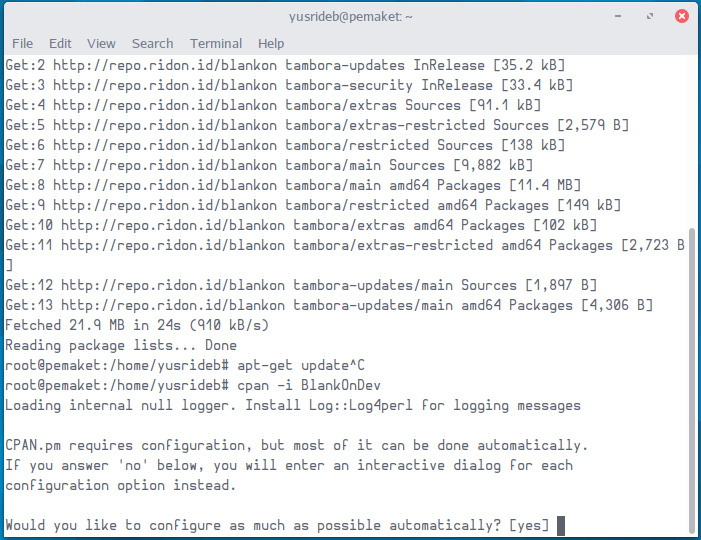
\includegraphics[width=10cm]{install-from-cpan-1.png}
	\caption{Form awal CPAN}
	\label{fig:bab2_form_awal_cpan}
\end{figure}

\noindent
Jika tampilkan form seperti gambar diatas, langsung saja tekan \textbf{Enter}.

\noindent
Jika sebelumnya anda sudah menggunakan perintah \textbf{\texttt{cpan -i}} maka instalasi module Perl akan dimulai, seperti berikut :

\begin{figure}[H]
	\centering
	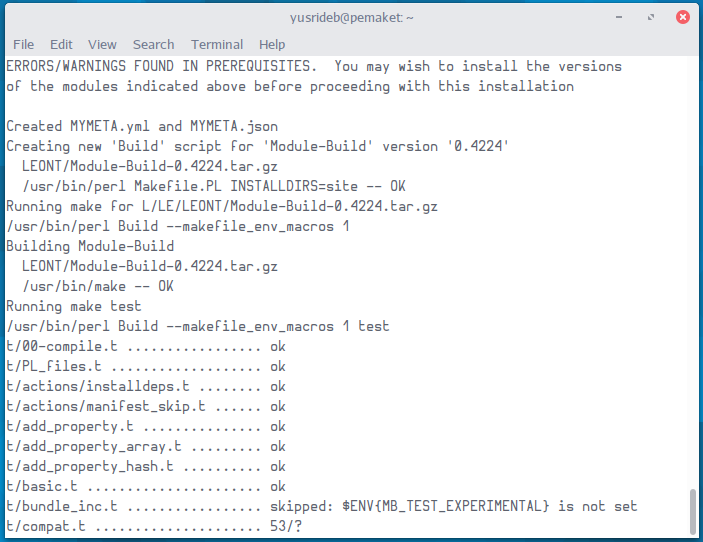
\includegraphics[width=9cm]{install-from-cpan-2.png}
	\caption{Instalasi Module Perl di mulai}
	\label{fig:bab2_start_install_module}
\end{figure}

\noindent
Jika dalam proses instalasi tidak ada yang bermasalah, maka akhir dari proses ini akan tampil seperti gambar berikut :

\begin{figure}[H]
	\centering
	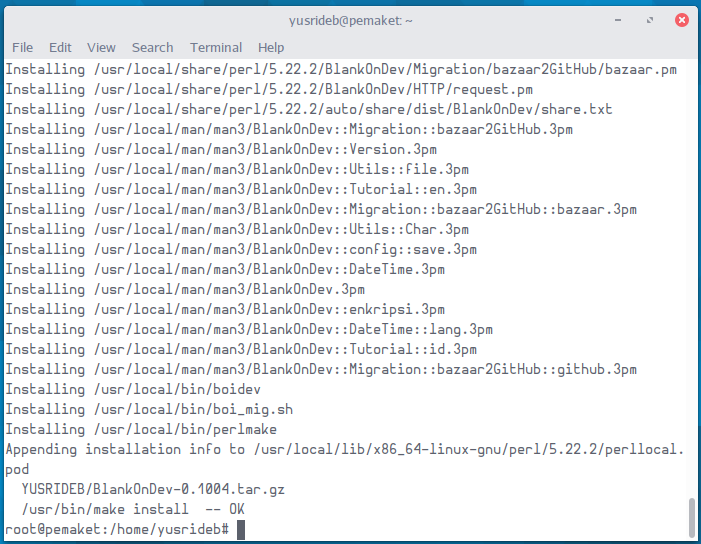
\includegraphics[width=9cm]{install-from-cpan-3_finish.png}
	\caption{Instalasi Module Selesai}
	\label{fig:bab1_finish_install_module}
\end{figure}

\pagebreak
\section{Implementasi}
\label{subsec:implm}
\noindent
Pada bagian ini akan dijelaskan langkah-langkah penggunaan perintah \textbf{boidev}. Berikut gambaran penggunaan perintah \textbf{boidev} :

\subsection{Persiapan Migrasi Paket :}
\begin{enumerate}
	\item \textbf{Step 1} - Perintah yang dijalankan sebelum menjalankan perintah \textbf{boidev} lainnya yaitu perintah \textbf{\texttt{boidev config}} untuk konfigurasi program seperti :
	\label{itm:pre_step1}
	\begin{itemize}
		\item Memasukkan nama \textbf{time zone},
		\item Memasukkan alamat \textbf{Email} yang digunakan di akun \textit{Github} dan maupun alamat \textbf{Email} untuk generate key dengan GnuPG, dan
		\item Generate Key GnuPG.
	\end{itemize}
	
	\item \textbf{Step 2} - Menggunakan perintah \texttt{boidev mig\_prepare}. Perintah ini akan melakukan persiapan sebelum Migrasi paket, yaitu :
	\label{itm:pre_step2}
	\begin{itemize}
		\item Config github, seperti \textit{nama}, \textit{Alamat Email}, dan \textit{Cache Username dan Password}
		
		\item Opsi Generate Key GnuPG.
		
		\item Memasukkan alamat bazaar repositori\\ (example: \textbf{http://dev.blankonlinux.or.id/browser/tambora}).
		
		\item Memasukkan alamat github repositori\\ (example: \textbf{https://github.com/blankon-packages})	
	\end{itemize}
	
	\item \textbf{Step 3} -  Menambahkan \textit{Group Paket} untuk \textit{Paket-paket} yang akan di migrasi ke repositori github. Perintah yang digunakan antara lain :
	\label{itm:pre_step3}
	\begin{enumerate}
		\item perintah \texttt{boidev bzr2git addpkg-group},
		\item perintah \texttt{boidev bzr2git addpkg} dan
		\item perintah \texttt{boidev bzr2git addpkg-file}
	\end{enumerate}
\end{enumerate}

\subsection{Proses Migrasi Paket :}
\begin{enumerate}
	
	\item \textbf{Skema split} - Branch, convert format, dan push dilakukan terpisah, dengan perintah :
	\label{itm:metode_split}
	\begin{enumerate}
		\item perintah \texttt{boidev bzr2git branch}
		\item perintah \texttt{boidev bzr2git bzr-cgit}
		\item perintah \texttt{boidev bzr2git git-push}
		\item perintah \texttt{boidev bzr2git git-check}
	\end{enumerate}
	
	\item \textbf{Skema one-time} - Branch, convert format, dan push dilakukan sekaligus dengan satu perintah yaitu dengan perintah \texttt{boidev bzr2git}.
	\label{itm:metode_one-time}
\end{enumerate}

\section{Persiapan Migrasi Paket}
\subsection{Persiapan Migrasi Paket - \texttt{boidev config}}
\label{implm_1}
\noindent
Jalankan perintah \texttt{boidev config} pada \textbf{User biasa} bukan \textit{User root} seperti berikut :

\begin{lstlisting}[language=ShellBash]
$ boidev config
\end{lstlisting}

\noindent
Kemudian proses \texttt{apt-get update} akan berjalan seperti berikut :

\begin{lstlisting}[language=ShellBash]

Hit:1 http://repo.ridon.id/blankon tambora InRelease
Hit:2 http://repo.ridon.id/blankon tambora-updates InRelease
Hit:3 http://repo.ridon.id/blankon tambora-security InRelease
Reading package lists... Done                      
Reading package lists... Done

\end{lstlisting}

\noindent
Setelah proses diatas maka akan di install beberapa paket-paket yang dibutuhkan oleh \textbf{Tim Pemaket}. Setelah instalasi paket selesai, Kemudian akan tampil Form seperti berikut dan masukkan nomor sesuai dengan yang ada di \textbf{List}.

\begin{lstlisting}[language=ShellBash]

List TimeZone : 
1. WIB 
2. WITA 
3. WIT 
Enter your time zone [WITA] : 2

\end{lstlisting}

\noindent
Form berikut ini isi sesuai petunjuk yang diberi tanda \textbf{\#}.

\begin{lstlisting}[language=ShellBash]

# Nama Lengkap
Enter your name : Achmad Yusri Afandi

# Email Github
Enter your email address Github Account : linuxer08@gmail.com

# Email yang digunakan saat generate GnuPG
Enter your email address for GnuPG Generate Key : yusrideb@cpan.org


# Masukkan Passphrase seperti saat menjalankan gpg --gen-key
Enter Passphrase gpg : 

# Untuk Cache username dan password github
# setelah username dan password dimasukkan pada saat 
# proses "git push"
You want to cache username and password github ? [y or n] y

\end{lstlisting}

\subsection{Dengan perintah \texttt{boidev mig\_prepare}}
\label{implm_2}
\noindent
Jalankan perintah berikut :

\begin{lstlisting}[language=ShellBash]
$ boidev mig_prepare
\end{lstlisting}

\noindent Setelah itu akan tampil form seperti pada \texttt{boidev config} :

\begin{lstlisting}[language=ShellBash]

List TimeZone : 
1. WIB 
2. WITA 
3. WIT 
Enter your time zone [WITA] : 2

\end{lstlisting}

\noindent
Form berikut yaitu form \textbf{Github config} :

\begin{lstlisting}[language=ShellBash]
You want reconfig github [y/n]:
\end{lstlisting}

\subsubsection{Penjelasan form \textbf{reconfig github} :}

\begin{itemize}
	\item Jika inputnya \textbf{\texttt{y}} maka akan tampil form config github seperti berikut :
	
	\begin{lstlisting}[language=ShellBash]
	# Masukkan nama jika, ingin mengubah nama yang sudah
	# tersimpan pada system. Jika tidak langsung tekan Enter
	Enter your github fullname [Achmad Yusri Afandi] : 
	
	# Masukkan email github, jika ingin mengubah nama yang sudah
	# tersimpan pada system. Jika tidak langsung tekan Enter
	Enter your github email [linuxer08@gmail.com] : 
	
	# Jika cache sudah aktif, maka form berikut akan tampil
	# jika cache belum aktif, maka form yang tampil yaitu :
	# "You want cache user and password git [y/n]:"
	# 
	# Jawaban hanya "y" or "n", jika dikosongkan 
	# maka sama dengan "n"
	You want to clear [y/n] : 
	\end{lstlisting}
	
	\item Jika inputnya \textbf{\texttt{n}} maka akan dilanjutkan ke form berikutnya.
\end{itemize}

\noindent
Form berikut yaitu form \textbf{Github config} clear cache atau aktifkan cache username dan passowrd github:

\begin{itemize}
	\item Jika cache aktif :
	\begin{lstlisting}[language=ShellBash]
	Cache user and password is activated
	You want to clear [y/n] : 
	\end{lstlisting}
	
	\item Jika cache belum aktif :
	\begin{lstlisting}[language=ShellBash]
	You want cache user and password git [y/n]: 
	\end{lstlisting}
\end{itemize}

\subsubsection{Form GnuPG Generate Key :}

\begin{lstlisting}[language=ShellBash]
You want cache user and password git [y/n]: 
\end{lstlisting}

\begin{itemize}
	\item Jika jawaban \textbf{\texttt{y}} :
	\begin{lstlisting}[language=ShellBash]
	# Masukkan nama jika, ingin mengubah nama yang sudah
	# tersimpan pada system. Jika tidak langsung tekan Enter
	Enter Name [Achmad Yusri Afandi] : 
	
	# Masukkan email untuk GnuPG, jika ingin mengubah nama yang
	# sudah tersimpan pada system. 
	# Jika tidak langsung tekan Enter
	Enter E-mail [yusrideb@cpan.org] : 
	\end{lstlisting}
	
	Setelah form disini, maka akan tampilk hasil \textbf{Generate Key GnuPG} :
	
	\begin{lstlisting}[language=ShellBash]
	You want to enter different passphrase GnuPG ? [y or n] y
	Enter passphrase : pub   1024R/243741DF 2017-06-12
	Key fingerprint = 8891 3EF3 6E21 C298 B7B6  0F0A 1380 3397 2437 41DF
	uid                  Achmad Yusri Afandi <yusrideb@cpan.org>
	sub   1024R/EF69A466 2017-06-12
	\end{lstlisting}
	
	\item Jika jawaban \textbf{\texttt{n}}, maka akan langsung ke form untuk memasukkan URL.
	
\end{itemize}

\subsubsection{Form URL Repositori Bazaar dan Github :}

\begin{itemize}
	\item Jika data \textbf{belum ada} :
	
	\begin{lstlisting}[language=ShellBash2]
	
	# Masukkan URL repositori bazaar, contohnya :
	# http://dev.blankonlinux.or.id/browser/tambora
	#
	Enter bzr url : 
	
	# Masukkan URL repositori Github, contohnya :
	# https://github.com/blankon-packages
	#
	Enter git url : 
	
	\end{lstlisting}
	
	\item Jika data \textbf{sudah ada} :
	
	\begin{lstlisting}[language=ShellBash2]
	
	# Masukkan URL  URL repositori bazaar jika anda ingin 
	# mengubah alamatnya. Jika tidak, langsung saja tekan Enter.
	#
	Enter bzr url [http://dev.blankonlinux.or.id/browser/tambora] : 
	
	# Masukkan URL  URL repositori github jika anda ingin 
	# mengubah alamatnya. Jika tidak, langsung saja tekan Enter.
	#
	Enter git url [https://github.com/blankon-packages] : 
	
	\end{lstlisting}
	
\end{itemize}

\subsection{Menambahkan Group paket dan nama paket}
\label{implm_3}
\noindent
Seperti yang telah dijelaskan pada upabab \textit{\ref{subsec:implm}. Implementasi - \textit{Persiapan Migrasi Paket}, di halaman \pageref{itm:pre_step3}} yaitu menggunakan perintah "\texttt{boidev bzr2git addpkg-group}", "\texttt{boidev bzr2git addpkg}" dan "\texttt{boidev bzr2git addpkg-file}".

\subsubsection{Menambahkan Group Paket}
\label{subsubsec:addpkg-group}
\noindent
Untuk menambahkan group paket ikut perintah berikut :

\begin{lstlisting}[language=ShellBash]
$ boidev bzr2git addpkg-group 
\end{lstlisting}

\noindent
kemudian akan tampil form seperti berikut :

\begin{lstlisting}[language=ShellBash]
Enter new group name : github-6
\end{lstlisting}

\noindent
Atau langsung masukkan nama paket group, contoh nama group paket \textbf{githb-6}

\begin{lstlisting}[language=ShellBash]
$ boidev bzr2git addpkg-group github-6
\end{lstlisting}

\noindent
Outputnya seperti berikut:

\begin{lstlisting}[language=ShellBash]

Success added package group with name "github-6"
\end{lstlisting}

\subsubsection{Melihat daftar Group paket}
\label{subsubsec:list-pkg-group}
\noindent
Jalankan perintah berikut :

\begin{lstlisting}[language=ShellBash]
$ boidev bzr2git list-pkg-group
\end{lstlisting}

\noindent
dan outputnya seperti berikut :

\begin{lstlisting}[language=ShellBash]

Exists Groups : 
------------------------------------------------------
- github-6

______________________________________________________
\end{lstlisting}

\subsubsection{Menambahkan nama paket}
\label{subsubsec:addpkg}
\noindent
Jalankan perintah berikut :

\begin{lstlisting}[language=ShellBash]
$ boidev bzr2git addpkg
\end{lstlisting}

\noindent
kemudian akan tampil form seperti berikut :

\begin{lstlisting}[language=ShellBash]
# Masukkan nomor list group
#
Choose Group Packages.
1. github-6
Enter Number choice : 1

# Masukkan nama group 
#
Enter New Packages : gnome-font-viewer
\end{lstlisting}

\noindent
atau langsung masukkan nama paket :

\begin{lstlisting}[language=ShellBash]
$ boidev bzr2git addpkg gnome-font-viewer
\end{lstlisting}

\noindent
Form pilih nama group :

\begin{lstlisting}[language=ShellBash]
# Masukkan nomor list group
#
Choose Group Packages.
1. github-6
Enter Number choice : 1
\end{lstlisting}

\subsubsection{Menambahkan nama paket dari file}
\label{subsubsec:addpkg-file}
\noindent
Cara ini digunakan jika terdapat lebih dari 1 nama paket yang akan ditambahkan contohnya :

\begin{lstlisting}[language=ShellBash]
gnome-documents
gnome-font-viewer
gnome-icon-theme
gnome-icon-theme-symbolic
gnome-keyring
gnome-logs
gnome-menus
gnome-music
gnome-online-accounts
gnome-packagekit
gnome-photos
gnome-pkg-tools
gnome-power-manager
gnome-screensaver
gnome-screenshot
gnome-shell
gnome-settings-daemon
gnome-shell-extensions
gnome-software
\end{lstlisting}

\noindent
Daftar nama paket tersebut dimasukkan kedalam file yang berekstensi \textbf{.boikg}, karena program hanya akan membaca file yang berekstensi \textbf{.boikg}

\noindent
Setelah daftar \textit{nama paket} dimasukkan dalam file, kemudian jalankan perintah berikut dengan syntax :\\ {\small \texttt{boidev bzr2git addpkg-file <lokasi\_file\/nama\_file.bokg>}}\\
Contoh lokasi file di : {\small \texttt{\/home\/yusrideb\/github-6.boikg}}

\begin{lstlisting}[language=ShellBash]
$ boidev bzr2git addpkg-file /home/yusrideb/github-6.boikg
\end{lstlisting}

\noindent
Kemudian akan tampil form untuk memilih group paket :

\begin{lstlisting}[language=ShellBash]
# Masukkan nomor list :
#
Choose Group Packages.
1. github-6
Enter Number choice : 1
\end{lstlisting}

\noindent
Output :

\begin{lstlisting}[language=ShellBash]

"gnome-documents" has success added.
"gnome-font-viewer" has success added.
"gnome-icon-theme" has success added.
"gnome-icon-theme-symbolic" has success added.
"gnome-keyring" has success added.
"gnome-logs" has success added.
"gnome-menus" has success added.
"gnome-music" has success added.
"gnome-online-accounts" has success added.
"gnome-packagekit" has success added.
"gnome-photos" has success added.
"gnome-pkg-tools" has success added.
"gnome-power-manager" has success added.
"gnome-screensaver" has success added.
"gnome-screenshot" has success added.
"gnome-shell" has success added.
"gnome-settings-daemon" has success added.
"gnome-shell-extensions" has success added.
"gnome-software" has success added.

19 packages has added...

\end{lstlisting}

\subsubsection{Melihat Daftar Paket}
\noindent
Untuk melihat list paket, menggunakan perintah : 
\begin{enumerate}
	\item {\small \texttt{boidev bzr2git list-pkg}}
	\item {\small \texttt{boidev bzr2git list-pkg <nama\_group\_paket>}}
\end{enumerate}

\noindent
\textbf{Perintah {\small \texttt{boidev bzr2git list-pkg}}}

\begin{lstlisting}[language=ShellBash]
$ boidev bzr2git list-pkg
\end{lstlisting}

\noindent
Kemudian akan form untuk memilih group paket, setelah itu akan tampil daftar paket seperti berikut:

\begin{figure}[H]
	\centering
	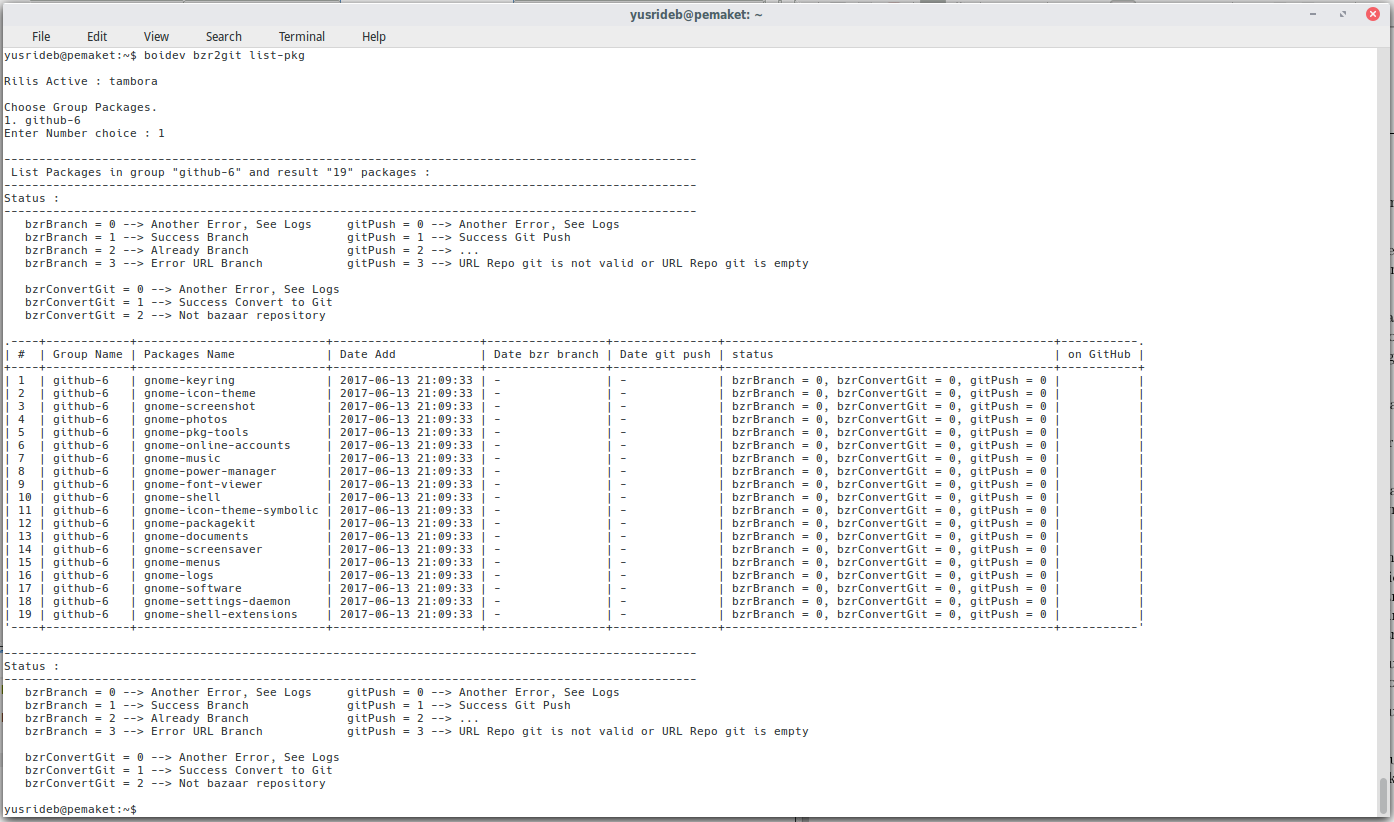
\includegraphics[width=12cm]{boidev_bzr2git_list-pkg.png}
	\caption{Daftar Paket yang telah ditambahkan dengan nama group \textbf{github-6}}
	\label{fig:bab2_list-pkg}
\end{figure}

\noindent
\textbf{Perintah {\small \texttt{boidev bzr2git list-pkg <nama\_group\_paket>}}}

\begin{lstlisting}[language=ShellBash]
$ boidev bzr2git list-pkg github-6
\end{lstlisting}

\noindent
Output :
\begin{figure}[H]
	\centering
	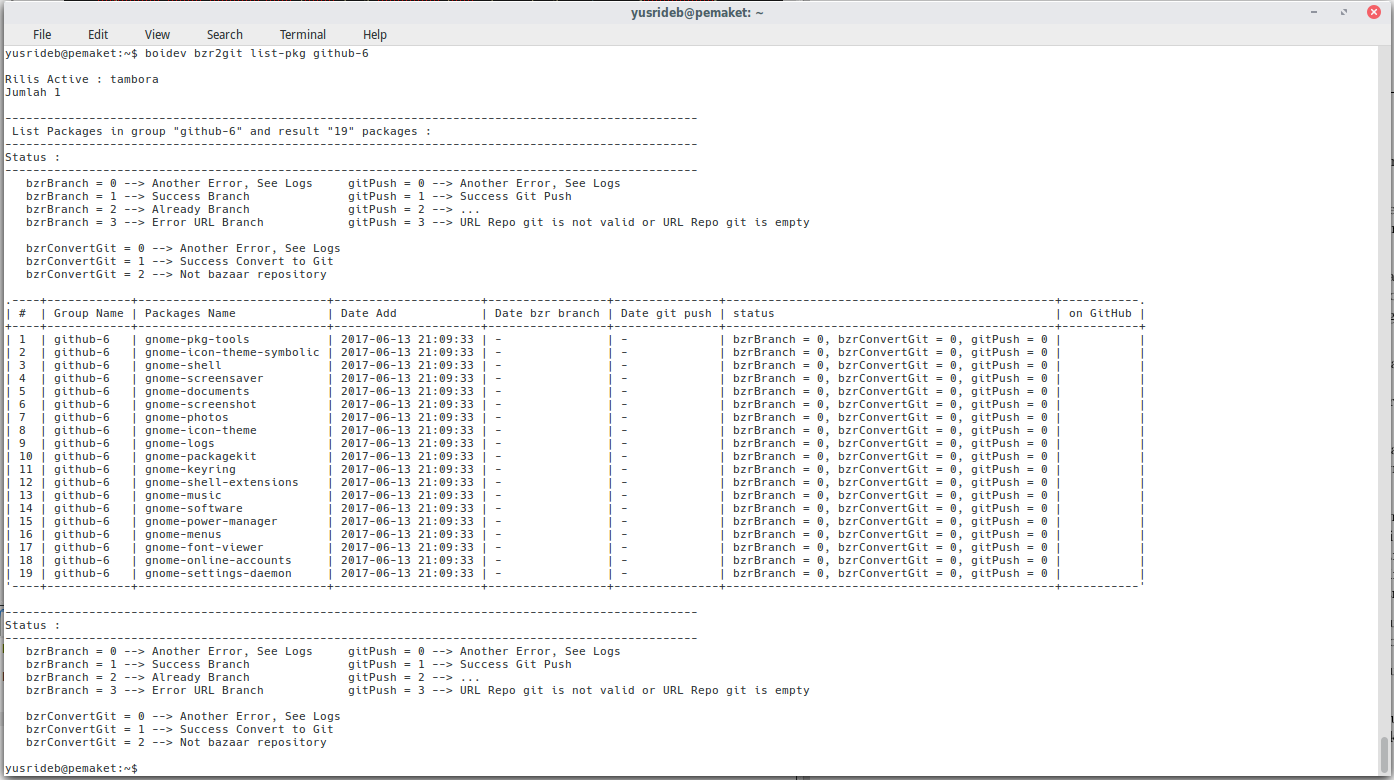
\includegraphics[width=12cm]{boidev_bzr2git_list-pkg_groupName.png}
	\caption{Daftar Paket yang telah ditambahkan dengan nama group \textbf{github-6}}
	\label{fig:bab2_list-pkg_bygrp}
\end{figure}

\section{Proses Migrasi Paket}
\label{sec:pre_impl_pros_mig}
\noindent
Proses yang dilakukan disini yaitu penggunaan perintah-perintah seperti contoh berikut, dengan perintah \textbf{boidev} yang lebih aman untuk meminimalisir kesalahan penulisan perintah ataupun kesalahan penulisan \textit{nama paket}.

\begin{lstlisting}[language=ShellBash2, caption=Perintah Migrasi, label=lst:migrasi_manual]

bzr branch http://dev.blankonlinux.or.id/browser/tambora/<nama_paket>
cd <nama_paket>
git init
bzr fast-export $(pwd) | git fast-import
git reset HEAD
rm -rf .bzr
git remote add origin git@github.com:blankon-packages/<nama_paket>.git
git push -u origin master
git checkout -b tambora
git push -u origin tambora
git branch -a
\end{lstlisting}

\subsection{Migrasi Paket dengan \textbf{Metode Split}}
\label{implm_4}
\noindent
Seperti yang telah dijelaskan pada upabab \textit{\ref{subsec:implm}. Implementasi, di halaman \pageref{itm:metode_split}}, Bahwa \textit{metode} ini melakukukan \textit{branch paket}, \textit{convert format ke git}, dan \textit{push ke git} secara terpisah. Seperti metode migrasi yang dilakukan secara manual seperti yang ditunjukkan pada \textit{listing - \ref{lst:migrasi_manual} Perintah Migrasi} diatas. Berikut langkah-langkahnya :

\subsubsection{Perintah {\small \texttt{boidev bzr2git branch}}}
\noindent
Perintah yang dapat digunakan yaitu :
\begin{itemize}
	\item {\small \texttt{boidev bzr2git branch}}
	\item {\small \texttt{boidev bzr2git branch <nama\_group\_paket>}}
\end{itemize}

\noindent
Proses yang akan tampil ketika salah satu perintah diatas dijalankan yaitu :

\begin{lstlisting}[language=ShellBash2]
# Masuk sesuai dengan nomor list
#
Choose Group Packages.
1. github-6
Enter Number choice : 1

# Jika jawabannya "y" maka jika nama paket sudah ada akan dihapus.
# Jika jawabannya "n" maka `branch` tidak akan dilakukan pada 
# nama paket yang sudah ada.
#
You want to re-branch if packages is exists on local directory [y/n] : y

Branch : "gnome-screensaver"
Result Action branch : 1


Branch : "gnome-icon-theme"
Result Action branch : 1

Branch : "gnome-menus"
Result Action branch : 1

Branch : "gnome-keyring"
Result Action branch : 1

Branch : "gnome-settings-daemon"
Result Action branch : 1

Branch : "gnome-online-accounts"
Result Action branch : 1

Branch : "gnome-shell-extensions"
Result Action branch : 1

Branch : "gnome-screenshot"
Result Action branch : 1

Branch : "gnome-font-viewer"
Result Action branch : 1

Branch : "gnome-logs"
Result Action branch : 1

Branch : "gnome-shell"
Result Action branch : 1

Branch : "gnome-music"
Result Action branch : 1

Branch : "gnome-icon-theme-symbolic"
Result Action branch : 1

Branch : "gnome-power-manager"
Result Action branch : 1

Branch : "gnome-documents"
Result Action branch : 1

Branch : "gnome-pkg-tools"
Result Action branch : 1

Branch : "gnome-software"
Result Action branch : 1

Branch : "gnome-photos"
Result Action branch : 1

Branch : "gnome-packagekit"
Result Action branch : 1

==================== bzr branch has finished ====================

\end{lstlisting}

\subsubsection{Perintah {\small \texttt{boidev bzr2git bzr-cgit}}}
\noindent
Perintah yang dapat digunakan yaitu :
\begin{itemize}
	\item {\small \texttt{boidev bzr2git bzr-cgit}}
	\item {\small \texttt{boidev bzr2git bzr-cgit <nama\_group\_paket>}}
\end{itemize}

\noindent
Proses yang akan tampil ketika salah satu perintah diatas dijalankan yaitu :

\begin{lstlisting}[language=ShellBash2]
# Masuk sesuai dengan nomor list
#
Choose Group Packages.
1. github-6
Enter Number choice : 1

Converting .... 

Action Convert gnome-logs : 1
Action Convert gnome-online-accounts : 1
Action Convert gnome-keyring : 1
Action Convert gnome-settings-daemon : 1
Action Convert gnome-screensaver : 1
Action Convert gnome-packagekit : 1
Action Convert gnome-power-manager : 1
Action Convert gnome-screenshot : 1
Action Convert gnome-font-viewer : 1
Action Convert gnome-music : 1
Action Convert gnome-icon-theme : 1
Action Convert gnome-software : 1
Action Convert gnome-shell : 1
Action Convert gnome-menus : 1
Action Convert gnome-pkg-tools : 1
Action Convert gnome-icon-theme-symbolic : 1
Action Convert gnome-documents : 1
Action Convert gnome-photos : 1
Action Convert gnome-shell-extensions : 1

======= Packages in group "github-6" has been finished to convert ========
\end{lstlisting}

\subsubsection{Perintah {\small \texttt{boidev bzr2git git-push}}}
\noindent
Perintah yang dapat digunakan yaitu :
\begin{itemize}
	\item {\small \texttt{boidev bzr2git git-push}}
	\item {\small \texttt{boidev bzr2git git-push <nama\_group\_paket>}}
\end{itemize}

\noindent
Proses yang akan tampil ketika salah satu perintah diatas dijalankan yaitu :

\begin{lstlisting}[language=ShellBash2]
# Masuk sesuai dengan nomor list
#
Choose Group Packages.
1. github-6
Enter Number choice : 1

Push to github .... 


gitpush : gnome-music

# Masukkan Username dan password github
#
Username for 'https://github.com': yusrideb
Password for 'https://yusrideb@github.com': 

\end{lstlisting}

\noindent
Jika username dan password github di cache sebelumnya, maka proses berikutnya tidak akan lagi meminta untuk memasukkan \textit{username dan password}.

\begin{lstlisting}[language=ShellBash2]
Action Git push for packages gnome-music : 1 
gitpush : gnome-software
Action Git push for packages gnome-software : 1 
gitpush : gnome-packagekit
Action Git push for packages gnome-packagekit : 1 
gitpush : gnome-icon-theme-symbolic
Action Git push for packages gnome-icon-theme-symbolic : 1 
gitpush : gnome-documents
Action Git push for packages gnome-documents : 1 
gitpush : gnome-power-manager
Action Git push for packages gnome-power-manager : 1 
gitpush : gnome-online-accounts
Action Git push for packages gnome-online-accounts : 1 
gitpush : gnome-settings-daemon
Action Git push for packages gnome-settings-daemon : 1 
gitpush : gnome-keyring
Action Git push for packages gnome-keyring : 1 
gitpush : gnome-font-viewer
Action Git push for packages gnome-font-viewer : 1 
gitpush : gnome-menus
Action Git push for packages gnome-menus : 1 
gitpush : gnome-screensaver
Action Git push for packages gnome-screensaver : 1 
gitpush : gnome-icon-theme
Action Git push for packages gnome-icon-theme : 1 
gitpush : gnome-shell
Action Git push for packages gnome-shell : 1 
gitpush : gnome-photos
Action Git push for packages gnome-photos : 1 
gitpush : gnome-screenshot
Action Git push for packages gnome-screenshot : 1 
gitpush : gnome-pkg-tools
Action Git push for packages gnome-pkg-tools : 1 
gitpush : gnome-shell-extensions
Action Git push for packages gnome-shell-extensions : 1 
gitpush : gnome-logs
Action Git push for packages gnome-logs : 1 

======= Packages in group "github-6" has been finished to git push =======
\end{lstlisting}

\subsubsection{Perintah {\small \texttt{boidev bzr2git git-check}}}
\noindent
Perintah yang dapat digunakan yaitu :
\begin{itemize}
	\item {\small \texttt{boidev bzr2git git-check}}
	\item {\small \texttt{boidev bzr2git git-check <nama\_group\_paket>}}
\end{itemize}

\noindent
Proses yang akan tampil ketika salah satu perintah diatas dijalankan yaitu :

\begin{lstlisting}[language=ShellBash2]
# Masuk sesuai dengan nomor list
#
Choose packages group : 
------------------------------------------------------
1. github-6                  [20]
------------------------------------------------------
Enter number of group name : 1

Check repo on github for all packages : 
Check Repo [gnome-music] on github : repo_github = master, tambora 
Check Repo [gnome-icon-theme-symbolic] on github : repo_github = master, tambora 
Check Repo [gnome-settings-daemon] on github : repo_github = master, tambora 
Check Repo [gnome-menus] on github : repo_github = master, tambora 
Check Repo [gnome-online-accounts] on github : repo_github = master, tambora 
Check Repo [gnome-shell-extensions] on github : repo_github = master, tambora 
Check Repo [gnome-documents] on github : repo_github = master, tambora 
Check Repo [gnome-keyring] on github : repo_github = master, tambora 
Check Repo [gnome-icon-theme] on github : repo_github = master, tambora 
Check Repo [gnome-power-manager] on github : repo_github = master, tambora 
Check Repo [gnome-logs] on github : repo_github = master, tambora 
Check Repo [gnome-photos] on github : repo_github = master, tambora 
Check Repo [gnome-shell] on github : repo_github = master, tambora 
Check Repo [gnome-font-viewer] on github : repo_github = master, tambora 
Check Repo [gnome-pkg-tools] on github : repo_github = master, tambora 
Check Repo [gnome-software] on github : repo_github = master, tambora 
Check Repo [gnome-screenshot] on github : repo_github = master, tambora 
Check Repo [gnome-screensaver] on github : repo_github = master, tambora 
Check Repo [gnome-packagekit] on github : repo_github = master, tambora 

======= Git Check All Packages on Group [github-6] has finished =======
\end{lstlisting}

\subsubsection{Melihat hasil Migrasi}
\noindent
Jika anda ingin melihat hasil migrasi gunakan perintah\\ {\small \texttt{boidev bzr2git list-pkg <nama\_group\_paket>}} seperti berikut :

\begin{lstlisting}[language=ShellBash]
$ boidev mig_prepare
\end{lstlisting}

\noindent
Output :

\begin{figure}[H]
	\centering
	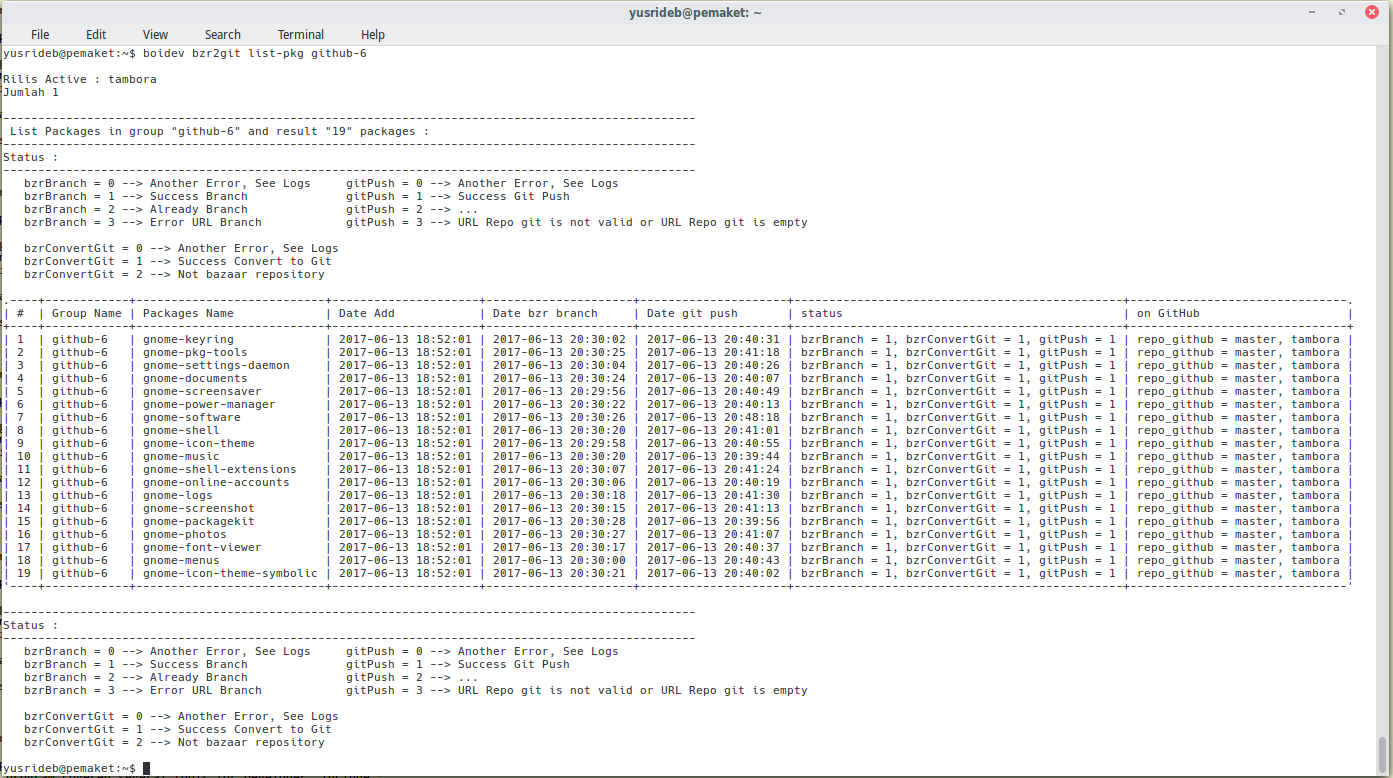
\includegraphics[width=13cm]{boidev_bzr2git_list-pkg-check.png}
	\caption{List Packages}
	\label{fig:bab2_list_pkg_check}
\end{figure}

\begin{figure}[H]
	\centering
	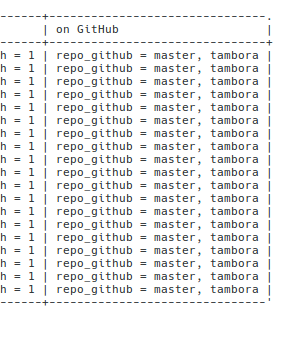
\includegraphics[width=5cm]{boidev_bzr2git_list-pkg-check_zoom.png}
	\caption{List Packages bagian hasil git-check}
	\label{fig:bab2_list_pkg_check_zoom}
\end{figure}

\subsection{Migrasi Paket dengan \textbf{Skema One-time}}
\label{implm_5}
\noindent 
Seperti yang telah dijelaskan pada upabab \textit{\ref{subsec:implm}. Implementasi, di halaman \pageref{itm:metode_one-time}}, Bahwa \textit{metode} ini melakukukan \textit{branch paket}, \textit{convert format ke git}, dan \textit{push ke git} sekaligus dengan perintah {\small \textit{\texttt{boidev bzr2git}}}. Skema ini menjalankan seluruh perintah yang terdapat pada \textit{listing - \ref{lst:migrasi_manual} Perintah Migrasi}, Berikut langkah-langkahnya:

\subsubsection{Migrasi 1 paket}

\begin{lstlisting}[language=ShellBash2]

# Untuk Migrasi 1 paket, maka masukkan nomor "3"
#
---------------------------------------------------------------------------
Choose Action : 
---------------------------------------------------------------------------
1. All Packages
2. Specific Group Packages
3. Single Packages
Answer: 3

# Contoh paket yaitu "gnome-keyring"
# 
Enter packages name : gnome-keyring

Branch : "gnome-keyring"
[success] Action "bzr branch -> gnome-keyring" : 1
[success] Action "bzr convert git -> gnome-keyring" 1
Username for 'https://github.com': yusrideb
Password for 'https://yusrideb@github.com': 
[success] Action "git push -> gnome-keyring" 1
[success] Action "git check -> gnome-keyring" repo_github = master, tambora

====== Migration packages "gnome-keyring" has been finished ======
\end{lstlisting}

\subsubsection{Migrasi Berdasarkan group paket}

\begin{lstlisting}[language=ShellBash2]

# Untuk Migrasi paket berdasarkan group, maka masukkan nomor "2"
#
---------------------------------------------------------------------------
Choose Action : 
---------------------------------------------------------------------------
1. All Packages
2. Specific Group Packages
3. Single Packages
Answer: 2

# Masukkan sesuai nomor list
# Pada contoh ini yaitu nomor "3"
#
Choose packages group : 
------------------------------------------------------
1. github-end-2              [10]
2. github-6                  [19]
3. github-end-3              [5]
4. github-end-1              [10]
------------------------------------------------------
Enter number of group name : 3

Doing migration ...

Branch : "ntfs-3g"
[success] Action "bzr branch -> ntfs-3g" : 1
[success] Action "bzr convert git -> ntfs-3g" 1
[success] Action "git push -> ntfs-3g" 1
[success] Action "git check -> ntfs-3g" repo_github = master, tambora
------------------------------------------------------------------------

Branch : "opencv"
[success] Action "bzr branch -> opencv" : 1
[success] Action "bzr convert git -> opencv" 1
[success] Action "git push -> opencv" 1
[success] Action "git check -> opencv" repo_github = master, tambora
------------------------------------------------------------------------
Branch : "nss"
[success] Action "bzr branch -> nss" : 1
[success] Action "bzr convert git -> nss" 1
[success] Action "git push -> nss" 1
[success] Action "git check -> nss" repo_github = master, tambora
------------------------------------------------------------------------
Branch : "nvidia-firmware"
[success] Action "bzr branch -> nvidia-firmware" : 1
[success] Action "bzr convert git -> nvidia-firmware" 1
[success] Action "git push -> nvidia-firmware" 1
[success] Action "git check -> nvidia-firmware" repo_github = master, tambora
------------------------------------------------------------------------
Branch : "notify-osd"
[success] Action "bzr branch -> notify-osd" : 1
[success] Action "bzr convert git -> notify-osd" 1
[success] Action "git push -> notify-osd" 1
[success] Action "git check -> notify-osd" repo_github = master, tambora
------------------------------------------------------------------------

======== Migration all packages in group "github-end-3" has been finished ========

\end{lstlisting}

\subsubsection{Migrasi Semua paket dalam list}

\begin{lstlisting}[language=ShellBash2]

# Untuk Migrasi semua paket, maka masukkan nomor "1"
#
---------------------------------------------------------------------------
Choose Action : 
---------------------------------------------------------------------------
1. All Packages
2. Specific Group Packages
3. Single Packages
Answer: 3

# Jika jawaban "y" maka semua paket yang terdaftar akan dimigrasi secara otomatis
# Jika jawaban "n" maka akan muncul pertanyaan sebelum paket dalam group di migrasi
# 
You want migration all packages with automatically ? [y or n] n

List Group packages to Migration : 
---------------------------------------------
1. github-end-1         [10]
2. github-end-2         [10]
3. github-6             [19]
4. github-end-3         [5]
---------------------------------------------

You want to migration all packages in group "github-end-1 [10]" ? [y or n] y

[migration] All packages in group "github-end-1" 
------------------------------------------------------------------------
Action re-branch for packages "live-boot" 
[success] Action "bzr branch -> live-boot" : 1
[success] Action "bzr convert git -> live-boot" 1
[success] Action "git push -> live-boot" 1
[success] Action "git check -> live-boot" repo_github = master, tambora
------------------------------------------------------------------------
Branch : "manokwari"
[success] Action "bzr branch -> manokwari" : 1
[success] Action "bzr convert git -> manokwari" 1
[success] re-Action "bzr convert git -> manokwari" 1
[success] Action "re-git push -> manokwari" 
[success] Action "git check -> manokwari" repo_github = master, tambora
------------------------------------------------------------------------
Branch : "linux-ntfs"
[success] Action "bzr branch -> linux-ntfs" : 1
[success] Action "bzr convert git -> linux-ntfs" 1
[success] Action "git push -> linux-ntfs" 1
[success] Action "git check -> linux-ntfs" repo_github = master, tambora
------------------------------------------------------------------------
Branch : "lvm2"
[success] Action "bzr branch -> lvm2" : 1
[success] Action "bzr convert git -> lvm2" 1
[success] Action "git push -> lvm2" 1
[success] Action "git check -> lvm2" repo_github = master, tambora
------------------------------------------------------------------------
Branch : "maleo"
[success] Action "bzr branch -> maleo" : 1
[success] Action "bzr convert git -> maleo" 1
[success] Action "git push -> maleo" 1
[success] Action "git check -> maleo" repo_github = master, tambora
------------------------------------------------------------------------
Branch : "mesa"
[success] Action "bzr branch -> mesa" : 1
[success] Action "bzr convert git -> mesa" 1
[success] Action "git push -> mesa" 1
[success] Action "git check -> mesa" repo_github = master, tambora
------------------------------------------------------------------------
Branch : "manokwari-theme"
[success] Action "bzr branch -> manokwari-theme" : 1
[success] Action "bzr convert git -> manokwari-theme" 1
[success] Action "git push -> manokwari-theme" 1
[success] Action "git check -> manokwari-theme" repo_github = master, tambora
------------------------------------------------------------------------
Branch : "live-config"
[success] Action "bzr branch -> live-config" : 1
[success] Action "bzr convert git -> live-config" 1
[success] Action "git push -> live-config" 1
[success] Action "git check -> live-config" repo_github = master, tambora
------------------------------------------------------------------------
Branch : "metacity"
[success] Action "bzr branch -> metacity" : 1
[success] Action "bzr convert git -> metacity" 1
[success] Action "git push -> metacity" 1
[success] Action "git check -> metacity" repo_github = master, tambora
------------------------------------------------------------------------
Branch : "manokwari-theme-greeter"
[success] Action "bzr branch -> manokwari-theme-greeter" : 1
[success] Action "bzr convert git -> manokwari-theme-greeter" 1
[success] Action "git push -> manokwari-theme-greeter" 1
[success] Action "git check -> manokwari-theme-greeter" repo_github = master, tambora
------------------------------------------------------------------------

You want to migration all packages in group "github-end-2 [10]" ? [y or n] n

[no-migration] All packages in group "github-end-2" 

You want to migration all packages in group "github-6 [19]" ? [y or n] y

[migration] All packages in group "github-6" 
------------------------------------------------------------------------
Action re-branch for packages "gnome-font-viewer" 
[success] Action "bzr branch -> gnome-font-viewer" : 1
[success] Action "bzr convert git -> gnome-font-viewer" 1
[success] Action "git push -> gnome-font-viewer" 1
[success] Action "git check -> gnome-font-viewer" repo_github = master, tambora
------------------------------------------------------------------------
Branch : "gnome-shell"
[success] Action "bzr branch -> gnome-shell" : 1
[success] Action "bzr convert git -> gnome-shell" 1
[success] Action "git push -> gnome-shell" 1
[success] Action "git check -> gnome-shell" repo_github = master, tambora
------------------------------------------------------------------------
Branch : "gnome-menus"
[success] Action "bzr branch -> gnome-menus" : 1
[success] Action "bzr convert git -> gnome-menus" 1
[success] Action "git push -> gnome-menus" 1
[success] Action "git check -> gnome-menus" repo_github = master, tambora
------------------------------------------------------------------------
Branch : "gnome-screensaver"
[success] Action "bzr branch -> gnome-screensaver" : 1
[success] Action "bzr convert git -> gnome-screensaver" 1
[success] Action "git push -> gnome-screensaver" 1
[success] Action "git check -> gnome-screensaver" repo_github = master, tambora
------------------------------------------------------------------------
Branch : "gnome-shell-extensions"
[success] Action "bzr branch -> gnome-shell-extensions" : 1
[success] Action "bzr convert git -> gnome-shell-extensions" 1
[success] Action "git push -> gnome-shell-extensions" 1
[success] Action "git check -> gnome-shell-extensions" repo_github = master, tambora
------------------------------------------------------------------------
Action re-branch for packages "gnome-power-manager" 
[success] Action "bzr branch -> gnome-power-manager" : 1
[success] Action "bzr convert git -> gnome-power-manager" 1
[success] Action "git push -> gnome-power-manager" 1
[success] Action "git check -> gnome-power-manager" repo_github = master, tambora
------------------------------------------------------------------------
Branch : "gnome-music"
[success] Action "bzr branch -> gnome-music" : 1
[success] Action "bzr convert git -> gnome-music" 1
[success] Action "git push -> gnome-music" 1
[success] Action "git check -> gnome-music" repo_github = master, tambora
------------------------------------------------------------------------
Branch : "gnome-online-accounts"
[success] Action "bzr branch -> gnome-online-accounts" : 1
[success] Action "bzr convert git -> gnome-online-accounts" 1
[success] Action "git push -> gnome-online-accounts" 1
[success] Action "git check -> gnome-online-accounts" repo_github = master, tambora
------------------------------------------------------------------------
Branch : "gnome-documents"
[success] Action "bzr branch -> gnome-documents" : 1
[success] Action "bzr convert git -> gnome-documents" 1
[success] Action "git push -> gnome-documents" 1
[success] Action "git check -> gnome-documents" repo_github = master, tambora
------------------------------------------------------------------------
Branch : "gnome-logs"
[success] Action "bzr branch -> gnome-logs" : 1
[success] Action "bzr convert git -> gnome-logs" 1
[success] Action "git push -> gnome-logs" 1
[success] Action "git check -> gnome-logs" repo_github = master, tambora
------------------------------------------------------------------------
Action re-branch for packages "gnome-keyring" 
[success] Action "bzr branch -> gnome-keyring" : 1
[success] Action "bzr convert git -> gnome-keyring" 1
[success] Action "git push -> gnome-keyring" 1
[success] Action "git check -> gnome-keyring" repo_github = master, tambora
------------------------------------------------------------------------
Branch : "gnome-icon-theme-symbolic"
[success] Action "bzr branch -> gnome-icon-theme-symbolic" : 1
[success] Action "bzr convert git -> gnome-icon-theme-symbolic" 1
[success] Action "git push -> gnome-icon-theme-symbolic" 1
[success] Action "git check -> gnome-icon-theme-symbolic" repo_github = master, tambora
------------------------------------------------------------------------
Branch : "gnome-screenshot"
[success] Action "bzr branch -> gnome-screenshot" : 1
[success] Action "bzr convert git -> gnome-screenshot" 1
[success] Action "git push -> gnome-screenshot" 1
[success] Action "git check -> gnome-screenshot" repo_github = master, tambora
------------------------------------------------------------------------
Branch : "gnome-photos"
[success] Action "bzr branch -> gnome-photos" : 1
[success] Action "bzr convert git -> gnome-photos" 1
[success] Action "git push -> gnome-photos" 1
[success] Action "git check -> gnome-photos" repo_github = master, tambora
------------------------------------------------------------------------
Action re-branch for packages "gnome-software" 
[success] Action "bzr branch -> gnome-software" : 1
[success] Action "bzr convert git -> gnome-software" 1
[success] Action "git push -> gnome-software" 1
[success] Action "git check -> gnome-software" repo_github = master, tambora
------------------------------------------------------------------------
Branch : "gnome-packagekit"
[success] Action "bzr branch -> gnome-packagekit" : 1
[success] Action "bzr convert git -> gnome-packagekit" 1
[success] Action "git push -> gnome-packagekit" 1
[success] Action "git check -> gnome-packagekit" repo_github = master, tambora
------------------------------------------------------------------------
Branch : "gnome-icon-theme"
[success] Action "bzr branch -> gnome-icon-theme" : 1
[success] Action "bzr convert git -> gnome-icon-theme" 1
[success] Action "git push -> gnome-icon-theme" 1
[success] Action "git check -> gnome-icon-theme" repo_github = master, tambora
------------------------------------------------------------------------
Branch : "gnome-settings-daemon"
[success] Action "bzr branch -> gnome-settings-daemon" : 1
[success] Action "bzr convert git -> gnome-settings-daemon" 1
[success] Action "git push -> gnome-settings-daemon" 1
[success] Action "git check -> gnome-settings-daemon" repo_github = master, tambora
------------------------------------------------------------------------
Branch : "gnome-pkg-tools"
[success] Action "bzr branch -> gnome-pkg-tools" : 1
[success] Action "bzr convert git -> gnome-pkg-tools" 1
[success] Action "git push -> gnome-pkg-tools" 1
[success] Action "git check -> gnome-pkg-tools" repo_github = master, tambora
------------------------------------------------------------------------

You want to migration all packages in group "github-end-3 [5]" ? [y or n] n

[no-migration] All packages in group "github-end-3" 

==================== Migration packages has been finished ====================

\end{lstlisting}